\documentclass[twoside]{report}
\usepackage{url}

\input{preamble}
\input{letterfonts}
\input{macros}






\definecolor{mycolor1}{HTML}{F3B47C}
\definecolor{mycolor2}{HTML}{A67F3A}


\newcommand*{\titre}[2]{\begingroup
	\newlength{\drop}
	\setlength{\drop}{0.1\textheight}
	\centering
	\settowidth{\unitlength}{\Huge\scshape CSS.317.1 Algorithmic Game Theory\hspace{3pt}-temps}
	\vspace*{\baselineskip}
	\rule{\unitlength}{1.6pt}\vspace*{-\baselineskip}\vspace*{2pt}
	\rule{\unitlength}{0.4pt}\\[\baselineskip]
	{\Huge\scshape\color{white} #1}\\[\baselineskip]
	{\large\itshape Instructor: #2}\\[\baselineskip]
	{\large\itshape TIFR 2025, Jan-May}\\[0.2\baselineskip]
	\rule{\unitlength}{0.4pt}\vspace*{-\baselineskip}\vspace{3.2pt}
	\rule{\unitlength}{1.6pt}\\[4\baselineskip]
	{\Large\scshape Scribe: Soham Chatterjee\\[10mm] soham.chatterjee@tifr.res.in \\[2mm] Website: \colorlink{black}{https://sohamch08.github.io/}{sohamch08.github.io} }\par
	\vfill
	% {\large\scshape\color{white} 2024}\par
	\endgroup}
	






\usepackage{xhfill}

\usetikzlibrary{calc} 

\titleformat{\chapter}[display]
{}
{\hfill \tikz[remember picture] \node[] (nr) {\fontsize{20}{70}\selectfont\color{mytoccolor}\textsc{Chapter~~} \fontsize{60}{70}\selectfont\color{mytoccolor}\thechapter};
	\begin{tikzpicture}[overlay,remember picture]
		\coordinate (rightborder) at ($(nr)+(100,0)$);
		\coordinate (right) at ($(nr.east) + (0.5,0)$);
		\draw[line width=4.5em] (right) -- (rightborder);
\end{tikzpicture}}
{-1ex}
{\filleft\fontsize{30}{50}\selectfont}
[\vspace{-1ex}]


\usetikzlibrary{arrows.meta, automata, calc,bending,positioning, quotes, overlay-beamer-styles}

\begin{document}

\pagestyle{plain}
%----------------------------------------------------------------------------------------
%	TITLE PAGE
%----------------------------------------------------------------------------------------
\thispagestyle{empty}



\begin{titlepage}

	\begin{tikzpicture}[remember picture,overlay]
		\node [xshift=\paperwidth/2,yshift=\paperheight/2] at (current page.south west)[minimum width=\paperwidth,minimum height=\paperheight,top color=mycolor1,bottom color=mycolor2]{};
	\end{tikzpicture}\\[3\baselineskip]

	\titre{CSS.317.1 Algorithmic Game Theory}{Umang Bhaskar}
\end{titlepage}



\newpage

	\pagestyle{plain}
\titleformat{name=\chapter,numberless}[display]
{\normalfont\Huge\bfseries}{}{0pt}{\Huge}
{\hypersetup{linkcolor=mytoccolor}
	\tableofcontents
	
}
\clearpage
\pagestyle{fancy}

%%%%%%%%%%%%%%%%%%%%%%%%%%%%%%%%%%%%%%
%%%%%%% Body
%%%%%%%%%%%%%%%%%%%%%%%%%%%%%%%%%%%%%%
%\setcounter{page}{1}
\include{chapters/equilibriums}
\include{chapters/bimatrix-game}
\include{chapters/complexity-class}
\chapter{Dynamics and Coarse Correlated Equilibrium}
\chapter{Potential Games}
\section{Best Response Dynamics}
The existence of a Nash equilibrium is clearly a desirable property of a strategic game. In this chapter and the next we discuss some natural classes of games that do have a Nash equilibrium. The \textit{Best-Response-Dynamics} is a straightforward procedure by which players search for a pure
Nash equilibrium ($\pne$) of a game. 

\begin{algorithm}\DontPrintSemicolon
\Begin{
\For{$t=1,\dots, T$}{
	\If{$t=1$}{Each player plays an arbitrary pure strategy}
	\Else{Pick a player $i\in[n]$\;
	$s_i^t\longleftarrow \arg\min\limits_{s_i\in S_i}c_i(s_i,s_{-i}^{t-1})$\;
$s_j^t\longleftarrow s_j^{t-1}\ \forall\ j\in[n]$, $j\neq i$}
}
}
	
\caption{\textsc{Best-Response-Dynamics} (\textsf{BRD})}
\end{algorithm}


\nt{Best-response dynamics can only halt at a $\pne$ and it cycles in any game without one. It can also cycle in games that have a $\pne$. For example consider the following 2 player.}

\section{Network (Atomic) Congestion Games}
\begin{definition}{Network (Atomic) Congestion Games}{}
	A network (atomic) congestion game or in short NCG consists of the following:
	\begin{itemize}[itemsep=-1mm]
		\item A directed graph $G=(V,E)$.
		\item $N$ players where  each player $i\in[n]$ has some source-sink pair $(s_i,t_i)\in V\times V$ associated with it.
		\item Edge cost functions $c_e:[n]\to \bbR$ for each edge $e\in E$.
		\item Player $i\in[N]$ has strategy set $S_i=$ Set of all $s_i\rightsquigarrow t_i$ paths in $G$. $S=\bigtimes\limits_{i=1}^N S_i$.
		\item For a strategy profile $f\in S$ (often called \textit{flow}), let $n_e(f)=|\{i\colon e\in f_i\}|$. Then the cost to player $i$ of strategy profile $f$ is $C_i(f)=\sum\limits_{e\in s_i}c_e(n_e(f))$. 
	\end{itemize}
\end{definition}

So we can define (atomic) NCG by the tuple $$\Big(G=(V,E),N,\{(s_i,t_i)\mid i\in[N]\}, \{c_e:[N]\to \bbR_{\geq 0}\mid e\in E\}\Big)$$

Note that unlike the last few lectures where we’ve been talking about utility-maximization games,
this is a \hyperref[def:cost-min-game]{cost-minimization game}. But of course we could just let a player’s utility be the negative
of its cost and everything would work as you expect.
\begin{lemma}{}{ncg-pne}
	Every NCG has a $\pne$.
\end{lemma}
\begin{proof}
	Given a strategy profile $f\in S$, we will define a potential function $\Phi:S\to\bbR_{\geq 0}$ with the property that if $f$ is not an equilibrium then $\exs\ f'\in S$ such that $\Phi(f)>\Phi(f')$. Thus if $f^*\in S$ minimizes $\Phi$ then $f^*$ must be a $\pne$.
	
	Consider the potential function $\Phi:S\to\bbR_{\geq 0}$: $$\Phi(s)=\sum_{e\in E}\sum_{i=1}^{n_e(f)}c_e(i)$$Now it is enough to calculate the change in potential when a player deviates to any other strategy since for $f,f'\in S$ $$\Phi(f)-\Phi(f')=\sum_{i=0}^{N-1} \Phi(f^{(i)})-\Phi(f^{(i+1)})$$ where $f^{(i)}=(f_1',f_2',\dots, f_i',f_{i+1},\dots, f_N)$ and for $f^{(0)}=f$. Now for any strategy profile $f\in S$ if the player $i$ deviates to the strategy $f_i'\in S_i$ then \begin{align*}
		C_i(f)-C_i(f'_i,f_{-i}) & = \lt[  \sum_{e\in f_i\cap f_i'}c_e(n_e(f))+\sum_{e\in f_i\setminus f_i'}c_e(n_e(f))\rt]-\lt[  \sum_{e\in f_i\cap f_i'}c_e(n_e(f_i',f_{-i}))+\sum_{e\in f_i'\setminus f_i}c_e(n_e(f_i',f_{-i}))\rt]\\
		&=  \sum_{e\in f_i\cap f_i'}\underbrace{c_e(n_e(f))-c_e(n_e(f_i',f_{-i}))}_{=0} + \sum_{e\in f_i\setminus f_i'}c_e(n_e(f))-\sum_{e\in f_i'\setminus f_i}c_e(n_e(f_i',f_{-i}))\\
		& = \sum_{e\in f_i\setminus f_i'}c_e(n_e(f))-\sum_{e\in f_i'\setminus f_i}c_e(n_e(f)+1)\\
	\end{align*}Therefore the change in the potential is \begin{align*}
	\Phi(f)-\Phi(f_i',f_{-i}) & = \sum_{e\in E}\sum_{i=1}^{n_e(f)} c_e(i)-\sum_{e\in E}\sum_{i=1}^{n_e(f_i',f_{-i})} c_e(i)\\
	& =\sum_{e\in E}\lt[\sum_{i=1}^{n_e(f)} c_e(i)-\sum_{i=1}^{n_e(f_i',f_{-i})} c_e(i)\rt]\\
	&=\sum_{e\in f_i\setminus f_i'}c_e(n_e(f))-\sum_{e\in f_i'\setminus f_i}c_e(n_e(f)+1)\\
	& = C_i(f)-C_i(f'_i,f_{-i})
\end{align*}So the change in potential is exactly equal to the change in the cost of the player who deviates. Therefore if $f$ is not a $\pne$ then $\exs\ i\in[N]$ such that $\exs\ f_i'\in S_i$ such that $c_i(f)-c_i(f_i',f_{-i})>0$ and therefore $\Phi(f)-\Phi(f_i',f_{-i})>0$. Hence every NCG has a $\pne$.
\end{proof}

\section{Potential Games}
\begin{definition}{Potential Game}{}
	A game $\Gm$ is a potential game if there exists a potential function $\Phi:S\to\bbR_{\geq 0}$ where $S$ is the set of strategy profiles such that $\forall\ s\in S$ and $s_i'\in S_i$ $C_i(s)-C_i(s_i',s_{-i})=\Phi(s)-\Phi(s_i',s_{-i})$
\end{definition}
 
 In the proof of \thmref{ncg-pne} we showed that every NCG is a potential game. Now we will show that every potential game has a $\pne$.
 \begin{Theorem}{}{}
 	Every potential game has a Pure Nash Equilibrium
 \end{Theorem}
\begin{proof}
	For a potential game $\Gm$ let $\Phi$ is the potential function for $\Gm$. Then $C_i(s)-C_i(s_i',s_{-i})=\Phi(s)-\Phi(s_i',s_{-i})$. Now consider the strategy profile $s=\arg\min\limits_{s\in S}\Phi(s)$. If any player had incentive to deviate there would be a strategy profile with smaller potential which is not possible by the definition of $s$. Therefore $s$ also has the minimum cost. Therefore $s$ is $\pne$. 
\end{proof}

\begin{lemma}{}{}
	Best Response Dynamics cannot cycle in a potential game.
\end{lemma}
\begin{proof}
	In each iteration of the $\brd$ every time any player deviates to play a best response the potential must decrease. Hence $\brd$ cannot cycle.
\end{proof}

Suppose there exists a time $T$ such that every player was chosen in the $\brd$ to choose their best response in the Best response algorithm. Then:
\begin{lemma}{}{}
	Let $s^*\in S$ be the strategy profile at time $t$. If $s^*$ is the strategy profile after $T$ further steps of $\brd$ then $s^*$ is a $\pne$.
\end{lemma}
\begin{proof}
	Since in every $T$ steps every player has the option to deviate to another strategy but chose not to. Therefore for each player $i\in[N]$, for all $s_i'\in S_i$, $C_i(s)\leq C_i(s_i',s_{-i})$. Therefore clearly $s^*$ is a $\pne$. 
\end{proof}
\begin{lemma}{}{}
	Let $s^\in S$ be the strategy profile after $T|S|$ steps of $\brd$. Then $s^*$ is a $\pne$.
\end{lemma}
\begin{proof}
	Since $\brd$ cannot cycle, $\exs\ s\in S$ that must have persisted fro $T$ time steps. Therefore by the previous lemma this must be a $\pne$.
\end{proof}

\begin{Theorem}{}{}
	In a finite potential game from an arbitrary initial outcome the Best Response Dynamics converges to a $\pne$ if $\exs\ T\in\bbN$ such that in every $T$ steps of $\brd$ every player is chosen at least once.
\end{Theorem}

Since every (Atomic) NCG is a potential game we have the following corollary:
\begin{corolary}{}{}
	In an (Atomic) NCG, $\brd$ converges to a $\pne$ if $\exs\ T\in\bbN$ such that in every $T$ steps of $\brd$ every player is chosen at least once. or ``every player is chosen infinitely often".
\end{corolary}


\subsection{General Congestion Games}
General Congestion Games are generalized version of (atomic) NCG. We will show that they are also potential game.
\begin{definition}{General Congestion Games}{}
	A basic definition general Congestion Games or CG consists of the following: $$\Big(E,N, \{S_i\mid i\in[N]\}, \{c_e:[N]\to \bbR_{\geq 0}\mid e\in E\}\Big)$$
	\begin{itemize}[itemsep=-1mm]
		\item A base set $E$ of congestible elements.
		\item $N$ players.
		\item For each player $i\in[N]$ a finite set of strategies $S_i$ where $S_i\subseteq 2^E$. $S=\bigtimes\limits_{i=1}^N S_i$.
		\item Cost functions $c_e:[N]\to \bbR$ for each element $e\in E$.
		\item For a strategy profile $s\in S$ (often called \textit{flow}), let $n_e(s)=|\{i\colon e\in s_i\}|$. Then the cost to player $i$ of strategy profile $s$ is $C_i(s)=\sum\limits_{e\in s_i}c_e(n_e(s))$. 
	\end{itemize}
\end{definition}

 Consider the  function $\Phi:S\to \bbR_{\geq 0}$ where for any strategy profile $s\in S$, $$\Phi(s)=\sum\limits_{e\in E}\sum\limits_{i=1}^{n_e(s)}c_e(i)$$ that is the same function as the potential function in the case of NCG. This is also a potential function for general CG's which makes general CG's are also potential game.
\subsection{Max Cut Game}

\begin{definition}{Max Cut Game}{}
	A max cut game consists of the following:
	\begin{enumerate}[itemsep=-1mm]
		\item An undirected weighted graph, $G=(V,E)$ and $w:E\to\bbR$.
		\item $N$ players.
		\item For each player $i\in[N]$, has 2 strategies: $S_i=\{L,R\}$. $S=\bigtimes\limits_{i=1}^N S_i$.	
		\item Utility functions $u_i:S\to \bbR_{\geq 0}$ for each player $i\in[N]$. For any strategy profile $s\in S$,  $u_i(s)=\sum\limits_{\substack{e=\{i,j\}\\ s_i\neq s_j}}w_e$
	\end{enumerate}
\end{definition}

So like general congestion games we can denote a Max Cut game by the tuple $(G,w,N)$. The max cut game is also a potential game. Consider the potential function $\Phi:S\to\bbR_{\geq 0}$ where for any strategy profile $s\in S$, $$\Phi(s)=\sum_{\substack{e=\{i,j\}\\ s)i\neq s_j}}w_e$$With this function we can prove that the Max Cut game is indeed a potential game and henceforth there exists a $\pne$.

\section{Class: \textsf{PLS}}
\begin{definition}{$\pls$ (Polynomial Local Search)}{}
	A local search problem $L$ has a set of problem instances $D_L\subseteq \Sg^*$ where any $I\in D_L$ is a particular problem instance. For each instance $I\in D_L$ there exists a finite solution set $F_L(I)\subseteq \Sg^*$. Let $R_L$ be the relation that models $L$ i.e. $$R_L\coloneqq \{(I,s)\mid I\in D_L,s\in F_L(I)\}$$ Then $R_L$ is in $\pls$ if:\begin{enumerate}[label=(\roman*)]
		\item The size of every solution $s\in F_L(I)$ for any $I\in D_L$ is polynomially bounded in the size of $I$.
		\item The problem instances $I\in D_L$ and the solutions $s\in F_L(I)$ are polynomial time verifiable.
		\item There is a polynomial time computable function $C_L:\Sg^*\times \Sg^*\to \bbR_{\geq 0}$ that returns for each $I\in D_L$ and each $s\in F_L(I)$ the cost $C_L(I,s)$.
		\item There is a polynomial time computable function $N:(I,s)\mapsto S$ where $S\subseteq F_L(I)$ i.e. returns the set of neighbors of lower cost for each $I\in D_L$ and each $s\in F_L(I)$ or states the $s$ is locally optimal.
	\end{enumerate}
\end{definition}

Note that for each $I\in D_L$ and each $s\in F_L(I)$ using (iii) and (iv) we can find a neighboring solutions of lower cost of $s$ or determine $s$ is locally minimal. The problem we want to focus is to find a locally minimal cost solution given an instance $I$ of $L$.

\begin{goal}
	Find a locally minimal cost solution given an instance $I$ of $L$.
\end{goal}
Finding $\pne$ in a Congestion Game (\textsf{PNE-CG}) is in $\pls$. Also finding $\pne $  in a Max Cut Game is in $\pls$.
\begin{lemma}{}{}
	$\textsf{PNE-CG}\in \pls$
\end{lemma}
\begin{proof}
	We will show that computing $\pne$ in congestion games is an instance of $\pls$ by fist describing conditions needed for $\pls$. Suppose $\Big(E,N, \{S_i\mid i\in[N]\}, \{c_e:[N]\to \bbR_{\geq 0}\mid e\in E\}\Big)$ be any instance of CG.
	\begin{enumerate}[label=(\roman*)]
		\item Any strategy profile is a solution for a specific instance of congestion games. Now each element of strategy profile by definition of CG is a subset of the base set $E$. Therefore size of any strategy profile is polynomially bounded by the size of the instance of the CG.
		\item For solution for the CG has to be valid strategy profile. So given any $N$-tuple of subsets of $E$ we can check if the $i^{th}$ element of the tuple is in $S_i$ for all $i\in[N]$ in polynomial time.
		\item For any strategy profile $s\in S$ we return the potential function for the CG as the cost function $\Phi(s)=\sum\limits_{e\in E}\sum\limits_{j=1}^{n_e(s)}c_e(i)$. This function is a polynomial time computable function.
		\item Given a strategy profile $s$ it checks if it is a $\pne$ by checking if we can switch the strategy of agent $i$ from $s_i$ to $s_i'$ such that $\Phi(s)>\Phi(s_i',s_{-i})$ for all agents.  If reduces then returns those strategy profiles. This is also polynomial time computable.
	\end{enumerate}
Therefore \textsf{PNE-CG} is in $\pls$.
\end{proof}
\begin{definition}{$\pls$-Reductions}{}
	A local search problem $L_1$ is $\pls$-reducible to another local search problem $L_2$, denoted by $L_1\leq_{\pls}L_2$ if there are two polynomial time computable functions $f:D_{L_1}\to D_{L_2}$ and $g:(I_1,s_2)\mapsto s_1$ where $I_1, D_{L_1}$, $s_2\in F_{L_2}(f(I_1))$ and $s_1\in F_{L_1}(I_1)$ such that:\begin{enumerate}[label=(\roman*)]
		\item If $I_1$ is an instance of $L_1$ then $f(I_1)$ is an instance of $L_2$
		\item If $s_2$ is an solution of $f(I_1)$ of $L_2$ then $g(I_1,s_2)$ is a solution for $I_1$ of $L_1$
		\item If $s_2$ is a local optimum for instance $f(I_1)$ of $L_2$ then $f(I_1,s_2)$ has to be a local optimum for instance $I_1$ of $L_1$.
	\end{enumerate}
\end{definition}
%https://panageas.github.io/agt22slides/Lecture9.pdf
\begin{Theorem}{}{}
	The Max Cut Game is $\pls$-complete
\end{Theorem}

We will not prove this but using this theorem we will prove the next theorem about general congestion games.

\begin{Theorem}{}{}
	General Congestion Games are $\pls$-complete
\end{Theorem}
\begin{proof}
	We already shown that general congestion games are in $\pls$. For completeness we will show a $\pls$-reduction from the Max Cut Game. Let $\Gm=(G,w,N)$ be an instance of a max cut game. We will create a congestion game $\Gm'=\Big(E',N, \{S_i\mid i\in[N]\}, \{c_e:[N]\to \bbR_{\geq 0}\mid e\in E\}\Big)$ with $N$ players.
	
	\begin{itemize}
		\item $E'$: For each edge $e\in E$ add two elements $e_L$ and $e_R$ to $E'$. So $E'=\{e_L,e_R\mid e\in E\}$.
		\item $S_i$: Each player $i\in[N]$ has two strategies $S_i=\lt\{\{e_L\mid e\text{ incident on $i$}\}, \{e_R\mid e\text{ incident on $i$}\}\rt\}$. Thus if $e=\{i,j\}\in E$ then the elements $e_L$, $e_R$ can be used by exactly 2 players $i$ and $j$ in $\Gm'$.
		\item $c_e:$ Define $c_{e_L}(1)=c_{e_R}(1)=0$ and $c_{e_L}(2)=c_{e_R}(2)=w(e)$.
	\end{itemize}
This defines a general congestion games. Now consider a strategy profile $s$ in $\Gm'$. Then $C_i(s)=\sum\limits_{\substack{j:\{i,j\}\in E\\ s_j\neq s_i}}e_{i,j}$. Therefore the local minimum in the $\Gm'$ gives a local minimum in $\Gm$. Hence max cut game is $\pls$-reducible to general congestion game.
\end{proof}
\chapter{Efficiency of Equilibria}
Here we are going to leave aside for now the question of how a game arrived at an equilibrium and instead we will study `\textit{quality of equilibria}'. We want to study how close to optimal the equilibria of a game are. But for that we have to define this `closeness' and `optimal'  by introducing cost to every strategy and we basically want to find a equilibria which very close to the minimum cost strategy profile.
\section{Cost Minimization Games}
\begin{Definition}{Cost Minimization Games}{cost-min-game}
	It is a game with $n$ players $[n]$, with their strategy sets $S_1,\dots, S_n$  where $S=\bigtimes\limits_{i=1}^n S_i$ and a cost function $C_i:S\to \bbR$ for each $i\in[n]$. 
\end{Definition}
 
There is an objective function $f:S\to \bbR$ with which the different strategy profiles are compared. There are many common choices for $f$. Conventionally the concepts $\pne$, $\mne$, $\ce$, $\cce$ are defined for utility-maximization games with all of its inequalities reversed. But the two Definitions are completely equivalent.\begin{itemize}
	\item \textbf{Pure Nash Equilibria}: A strategy profile $s\in S$ of a cost-minimization game $\Gm$ is a \textit{Pure Nash Equilibrium} if for every player $i\in[n]$ and for all $s'_i\in S_i$, $C_i(s)\leq C_i(s_i',s_{-i})$.
	\item \textbf{Mixed Nash Equilibria}: A mixed strategy profile $\sg\in \Sg$ of a cost-minimization game $\Gm$ is a \textit{Mixed Nash Equilibria} if for every player $i\in[n]$ and for all $s_i'\in S_i$, $\underset{s\sim \sg}{\bbE}[C_i(s)]\leq \underset{s\sim \sg}{\bbE}[C_i(s_i',s_{-i})]$
	\item \textbf{Correlated Equilibria}: A distribution $\mu$ over $S$ of a cost-minimization game $\Gm$ is a \textit{Correlated Equilibria} if for every player $i\in[n]$ and for all $s_i'\in S_i$, $\underset{s\sim \mu}{\bbE}[C_i(s)\mid s_i]\leq \underset{s\sim \mu}{\bbE}[C_i(s_i',s_{-i})\mid s_i]$
	\item \textbf{Coarse Correlated Equilibria}: A distribution $\mu$ over $S$ of a cost-minimization game $\Gm$ is a \textit{Coarse Correlated Equilibria} if for every player $i\in[n]$ and for all $s_i'\in S_i$, $\underset{s\sim \mu}{\bbE}[C_i(s)]\leq \underset{s\sim \mu}{\bbE}[C_i(s_i',s_{-i})]$
\end{itemize}

\section{Pareto Optimality}
\begin{Definition}{Pareto Optimal Strategy}{}
Given a game $\Gm$, a strategy profile $s\in S$	is pareto optimal also denoted by \textsf{PO} if $\not\exists\ s'\in S$ such that $$\forall\ i\in[n],\ c_i(s')\leq c_i(s)\qquad\exs\ i\in[n]\ c_i(s')<c_i(s)$$or equivalently for all $s'\in S$, either $\forall\ i\in[n]$, $c_i(s)=c_i(s')$ or $\exs\ i\in[n]$, $c_i(s')>c_i(s)$.
\end{Definition}

Economists call Pareto Optimality ``efficiency". \textsf{PO} induces a partial order over the set of all strategy profiles. Let $s,s'\in S$. We say that $s>_ps'$ if $\forall\ i\in[n],\ c_i(s')\leq c_i(s)$ and $\exs\ i\in[n]\ c_i(s')<c_i(s)$.

To introduce a total order we can think of  social welfare function for example:
\begin{enumerate}[label=(\arabic*)]
	\item Utilitarian Social Welfare: For any $s\in S$, $C(s)=\sum\limits_{i=1}^n c_i(s)$
	\item Nash Social Welfare: For any $s\in S$, $C(s)=\sum\limits_{i=1}^n c_i(s)$
	\item Egalitarian Social Welfare: For any $s\in S$, $C(s)=\max\limits_{i=1}^n c_i(s)$
\end{enumerate}This allows us to quantitatively see how good or bad a equilibrium is by comparing two strategy profiles. Typically by ``social welfare" we mean utilitarian social welfare. We will focus on calculating utilitarian social welfare from now on.
\section{Price of Anarchy}

For a game $\Gm$ we also want to know how bad is the social welfare at equilibrium compared to the best possible social welfare. This ratio is know as Price of Anarchy.
\begin{Definition}{Price of Anarchy}{}
	We denote it by $\poa$. For a game $\Gm$:\begin{align*}
		\poa(\Gm)& =\frac{\text{Social welfare of ``worst equilibrium"}}{\text{Optimal social welfare}}\\
		&= \frac{\max\lt\{\sum\limits_{i=1}^n C_i(s)\colon s\in S\text{ is an $\pne$}\rt\}}{\min\lt\{\sum\limits_{i=1}^n C_i(s)\colon s\in S\rt\}}
	\end{align*}
\end{Definition}
\subsection{\textsf{PoA} of Network (Atomic) Congestion Games}

\begin{Theorem}{}{poa-ncg}
	The $\poa$ in network congestion games with affine cost functions is $\frac{5}2$.
\end{Theorem}
\begin{proof}We will prove this in two stages. First we will show that the lower bound for $\poa$ for NCG is at least $\frac52$ by constructing an example. Then we will show the upper bound.\vspace*{2mm}
\parinf

\textbf{Lower Bound $\geq \frac52$:}
\vspace*{2mm}

\begin{minipage}{0.4\textwidth}
	\captionsetup{type=figure}
		\begin{center}
		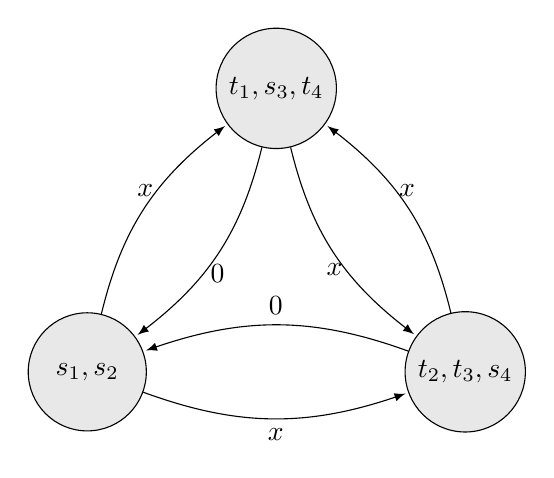
\begin{tikzpicture}[shorten >=1pt, auto,scale=0.8]
			\tikzstyle{every state}=[fill={rgb:black,1;white,10}, minimum size=1.5cm]
			
			% Arrange nodes with increased distance
			\node[state] (0) at (0, 3)                {$t_1,s_3,t_4$};
			\node[state] (1) at (-3, -1.5)               {$s_1,s_2$};
			\node[state] (2) at (3, -1.5)                {$t_2,t_3,s_4$};
			
			% Define all the edges with labels
			\path[-latex] (1) edge[bend right=20] node[below] {$x$} (2);
			\path[-latex] (2) edge[bend right=20] node[above] {$0$} (1);
			\path[-latex] (1) edge[bend left=20] node[above] {$x$} (0);
			\path[-latex] (0) edge[bend left=20] node[below] {$0$} (1);
			\path[-latex] (0) edge[bend right=20] node[below] {$x$} (2);
			\path[-latex] (2) edge[bend right=20] node[above] {$x$} (0);
		\end{tikzpicture}
	\end{center}
%\caption{NCG: $\poa$ Lower Bound}
\end{minipage}\hfill
\begin{minipage}{0.57\textwidth}
	Consider the NCG with 4 players drawn on the left. \parinn
	
	The optimal cost for this NCG is when every player uses the single-edge $s_i\to t_i$ paths. And the cost for each such path is $1$ as none of these 4 edges is used by more than 1 player. So the optimal value is $4$. Note that this is also a $\pne$.
	
	Now we will calculate the worst $\pne$. Every player uses the $2$-edge $s_i\to t_i$ paths. Then the costs for each players are 
	
		\begin{enumerate*}[label=\arabic*:, itemjoin={,\   }, itemjoin*={,\   }]
		\item 3
		\item 3
		\item 2
		\item 2
	\end{enumerate*}\parinf

Therefore total cost is $10$. Hence $\poa\geq \frac{10}4=\frac52$.
\end{minipage}

\newpage
\parinf

\textbf{Upper Bound $\leq \frac52$:}
\vspace*{2mm}
\begin{claimwidth}
\begin{lemma}{}{}
	For any NCG with $N$ players if $s$ is any strategy profile and $s^*$ is a $\pne$ then $C(s^*)\leq \frac52 C(s)$.
\end{lemma}
\begin{proof}
	For each player $i\in [N]$ we have 
	\[	C_i(s^*)  \leq C_i(s_i,s_{-i}^*) = \sum\limits_{e\in s_i\cap s_i^*}c_e(n_e(s^*))+\sum\limits_{e\in s_i\setminus s_i^*} c_e(n_e(s^*)+1)\leq \sum\limits_{e\in s_i}c_e(n_e(s^*)+1)\] Now summing over all players we get the total cost \begin{align*}
		C(s^*) =\sum\limits_{i\in[N]}c_i(s^*) & = \sum\limits_{i\in[N]}\sum\limits_{e\in s_i}c_e(n_e(s^*)+1)\\
		& =\sum\limits_{e\in E}c_e(n_e(s^*)+1)n_e(s)\\
		& = \sum\limits_{e\in E}\Big(a_e(n_e(s^*)+1)+b_e\Big)n_e(s)& [\text{Let $c_e(i)=a_ei+b_e$, $a_e,b_e\geq  0$}]\\
		& = \sum\limits_{e\in E}a_en_e(s)(n_e(s^*)+1)+b_en_e(s)\\
		& \leq \sum\limits_{e\in E}a_e\lt(\frac53n_e^2(s)+\frac13n_e^2(s^*)\rt)+b_en_e(s) & \lt[x,y\in\bbZ,x(y+1)\leq \frac53x^2+\frac13y^2\rt]\\
		& = \sum\limits_{e\in E}n_e(s)\lt(\frac53a_en_e(s)+b_e\rt)+\frac13a_en_e^2(s^*)\\
		& \leq \frac53\sum\limits_{e\in E}n_e(s)(a_en_e(s)+b_e)+\frac13 \sum\limits_{e\in E}n_e(s^*)(a_en_e(s^*)+b_e)\\
		& = \frac53C(s)+\frac13C(s^*) 
	\end{align*}
Therefore we get $$C(s^*)\leq \frac53C(s)+\frac13C(s^*)\implies \frac23C(s^*)\leq \frac53C(s)\implies C(s^*)\leq \frac52C(s)$$Hence we have the lemma.
\end{proof}
\end{claimwidth}


Using the lemma for any $\pne$ $s^*\in S$ and any strategy profile $s\in S$ we have $C(s^*)\leq \frac52C(s)$. Therefore the worst cost $\pne$ and the optimal strategy profile  also follows the inequality. Therefore the $\poa$ is at most $\frac52$. Therefore we get the upper bound also.
\end{proof}

\section{Global Connection Games}
\begin{Definition}{Global Connection Games}{}
	A Global Connection Games or in short GCG consists of the following:$$\Big(G=(V,E),N,\{(s_i,t_i)\mid i\in[N]\}, \{c_e \mid e\in E,c_e\geq 0\}\Big)$$
	\begin{itemize}[itemsep=-1mm]
		\item A directed graph $G=(V,E)$.
		\item $N$ players where  each player $i\in[n]$ has some source-sink pair $(s_i,t_i)\in V\times V$ associated with it.
		\item Edge costs $c_e$ for each edge $e\in E$ where $c_e\geq 0$.
		\item Player $i\in[N]$ has strategy set $S_i=$ Set of all $s_i\rightsquigarrow t_i$ paths in $G$. $S=\bigtimes\limits_{i=1}^N S_i$.
		\item For a strategy profile $f\in S$, let $n_e(f)=|\{i\colon e\in f_i\}|$. Then the cost to player $i$ of strategy profile $f$ is $C_i(f)=\sum\limits_{e\in s_i}\frac{c_e}{n_e(f)}$ i.e. the cost of edge is divides equally among all the players using that edge.
	\end{itemize}
\end{Definition}

Therefore for any strategy profile the total cost is $$C(f)=\sum\limits_{i\in[N]}C_i(f)=\sum\limits_{i\in[N]}\sum\limits_{e\in s_i}\frac{c_e}{n_e(s)}=\sum\limits_{\substack{e\in E\\ n_e(f)>0}}c_e$$

\begin{lemma}{}{}
	GCG is a potential game
\end{lemma}
\begin{proof}
	Consider the function $\Phi:S\to \bbR_{\geq 0}$ where for any strategy profile $f\in S$  $$\Phi(f)=\sum\limits_{e\in E}\sum\limits_{j=1}^{n_e(f)}\frac{c_e}{j}=\sum\limits_{\substack{e\in E\\ n_e(f)\geq 1}}c_eH_{n_e(s)}$$where $H_n$ is the $n^{th}$ harmonic number. Then we  have for any $f\in S$ and $f_i'\in S_i$ \begin{align*}
		\Phi(f)-\Phi(f_i',f_{-i}) & =\sum\limits_{e\in E}\sum\limits_{j=1}^{n_e(f)}\frac{c_e}{j}-\sum\limits_{e\in E}\sum\limits_{j=1}^{n_e(f_i',f_{-i})}\frac{c_e}{j}      =\sum\limits_{e\in E}\lt[\sum\limits_{j=1}^{n_e(f)}\frac{c_e}{j}-\sum\limits_{k=1}^{n_e(f_i',f_{-i})}\frac{c_e}{k}\rt]                                                                                                                                                         \\
		                          & = \sum\limits_{e\in E\setminus f_i\cup f_i'}\lt[\sum\limits_{j=1}^{n_e(f)}\frac{c_e}{j}-\sum\limits_{k=1}^{n_e(f_i',f_{-i})}\frac{c_e}{k}\rt]+\sum\limits_{e\in f_i\cap f_{i}'}\lt[\sum\limits_{j=1}^{n_e(f)}\frac{c_e}{j}-\sum\limits_{k=1}^{n_e(f_i',f_{-i})}\frac{c_e}{k}\rt]+\sum\limits_{e\in f_i\setminus f_i'}\lt[\sum\limits_{j=1}^{n_e(f)}\frac{c_e}{j}-\sum\limits_{k=1}^{n_e(f_i',f_{-i})}\frac{c_e}{k}\rt] \\
		                          & \qquad\qquad\qquad\qquad\qquad\qquad\qquad\qquad\qquad\qquad\qquad\qquad\qquad\qquad+\sum\limits_{e\in f_i'\setminus f_i}\lt[\sum\limits_{j=1}^{n_e(f)}\frac{c_e}{j}-\sum\limits_{k=1}^{n_e(f_i',f_{-i})}\frac{c_e}{k}\rt]                                                                                                                                                                                             \\
		                          & =\sum\limits_{e\in f_i\cap f_{i}'}\underbrace{\lt[\sum\limits_{j=1}^{n_e(f)}\frac{c_e}{j}-\sum\limits_{k=1}^{n_e(f_i',f_{-i})}\frac{c_e}{k}\rt]}_{0}+\sum\limits_{e\in f_i\setminus f_i'}\lt[\sum\limits_{j=1}^{n_e(f)}\frac{c_e}{j}-\sum\limits_{k=1}^{n_e(f_i',f_{-i})}\frac{c_e}{k}\rt] +\sum\limits_{e\in f_i'\setminus f_i}\lt[\sum\limits_{j=1}^{n_e(f)}\frac{c_e}{j}-\sum\limits_{k=1}^{n_e(f_i',f_{-i})}\frac{c_e}{k}\rt]\\
		                          &=\sum\limits_{e\in f_i\cap f_{i}'}\lt[\sum\limits_{j=1}^{n_e(f)}\frac{c_e}{j}-\sum\limits_{k=1}^{n_e(f_i',f_{-i})}\frac{c_e}{k}\rt]+\sum\limits_{e\in f_i\setminus f_i'}\frac{c_e}{n_e(f)} -\sum\limits_{e\in f_i'\setminus f_i}\frac{c_e}{n_e(f_i',f_{-i})} = C_i(f)-C_i(f_i',f_{-i})
	\end{align*}
Therefore GCG is a potential game.
\end{proof}
\begin{Theorem}{}{}
The $\poa$ for any GCG with $N$ players is $N$.
\end{Theorem}
\begin{proof}
Like the case for NCG we will prove this in two stages. First we will show that the lower bound for $\poa$ for GCG with $N$ players is at least $N$ by constructing an example. Then we will show the upper bound.\vspace*{2mm}
\parinf

\textbf{Lower Bound $\geq N$:}
\vspace*{2mm}

\begin{minipage}{0.4\textwidth}
	\captionsetup{type=figure}
	\begin{center}
		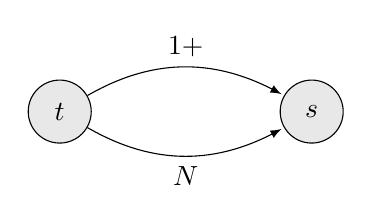
\begin{tikzpicture}[shorten >=1pt, auto,scale=0.8]
			\tikzstyle{every state}=[fill={rgb:black,1;white,10}, minimum size=0.8cm]
			
			% Arrange nodes with increased distance
			\node[state] (0) at (2,0)                {$s$};
			\node[state] (1) at (-2,0)               {$t$};
			
			% Define all the edges with labels
			\path[-latex] (1) edge[bend right=30] node[below] {$N$} (0);
			\path[-latex] (1) edge[bend left=30] node[above] {$1+\eps$} (0);

		\end{tikzpicture}
	\end{center}
	%\caption{NCG: $\poa$ Lower Bound}
\end{minipage}\hfill
\begin{minipage}{0.57\textwidth}
	Consider the GCG with 5 players drawn on the left where for each player $i\in[N]$, $s_i=s$ and $t_i=t$. \parinn
	
	The optimal cost for this GCG is when every player uses the edge with cost $1+\eps$. Hence the total cost is $1+\eps$.
	
	Now we will calculate the worst $\pne$. Every player uses the edge with cost $N$. Therefore total cost is $N$. Hence $\poa\geq \frac{N}{1+\eps}\geq N$.
\end{minipage}
\vspace*{2mm}

\textbf{Upper Bound $\leq N$:}
\vspace*{2mm}

Let $\Gm$ be any GCG. Suppose $s^*$ be any $\pne$ of $\Gm$ and $s_{\textsc{opt}}$ is the optimal strategy profile. \begin{claimwidth}
	\begin{claim}{}{}
		$C_i(s^*)\leq \text{cost}(s_{\textsc{opt}_i})$ where $\text{cost}(s_{\textsc{opt}_i})=\sum\limits_{e\in s_{\textsc{opt}_i}}c_e$.
	\end{claim}
\begin{proof}
	Suppose not. Then 	$C_i(s^*)> \text{cost}(s_{\textsc{opt}_i})$. Now we have $$C_i(s_{\textsc{opt}_i},s^*_{-i})=\sum\limits_{e\in s_{\textsc{opt}_i}}\frac{c_e}{n_e(s_{\textsc{opt}_i},s^*_{-i})}\leq  \sum\limits_{e\in s_{\textsc{opt}_i}}{c_e}=\text{cost}(s_{\textsc{opt}_i})$$Therefore we get $C_i(s^*)>C_i(s_{\textsc{opt}_i},s^*_{-i})$.   But $s^*$ is a $\pne$. Hence contradiction \ctr 
\end{proof}
\end{claimwidth}

Therefore we have $$C(s^*)=\sum\limits_{i\in[N]}C_i(s^*)\leq \sum\limits_{i\in[N]} \text{cost}(s_{\textsc{opt}_i})\leq \sum\limits_{i\in[N]}\sum\limits_{e\in s_{\textsc{opt}_i}}c_e\leq \sum\limits_{i\in[N]}\sum\limits_{e\in s_{\textsc{opt}_i}}N\cdot\frac{c_e}{n_e(s_{\textsc{opt}})}=N\sum\limits_{i\in[N]}C_i(s_{\textsc{opt}})=N\cdot C(s_{\textsc{opt}}) $$Hence we get that $\poa(\Gm)\leq N$.
\end{proof}

\section{Price of Stability}
In the case of GCG we can see that always comparing the worst Pure Nash Equilibria with the optimal strategy may lead to very large value. So instead sometimes we prefer to compare the best $\pne$ and the optimal strategy.
\begin{Definition}{Price of Stability}{}
	We denote it by $\pos$. For a game $\Gm$:\begin{align*}
		\pos(\Gm)& =\frac{\text{Social welfare of ``best equilibrium"}}{\text{Optimal social welfare}}\\
		&= \frac{\min\lt\{\sum\limits_{i=1}^n C_i(s)\colon s\in S\text{ is an $\pne$}\rt\}}{\min\lt\{\sum\limits_{i=1}^n C_i(s)\colon s\in S\rt\}}
	\end{align*}
\end{Definition}

\subsection{$\pos$ of Global Connection Games}
\begin{lemma}{}{}
	In a GCG with $N$ players the $\pos$ is at least $H_N$.
\end{lemma}
\begin{proof}
	We will prove this using an example of GCG.
	\vspace*{2mm}
	
	\begin{center}
			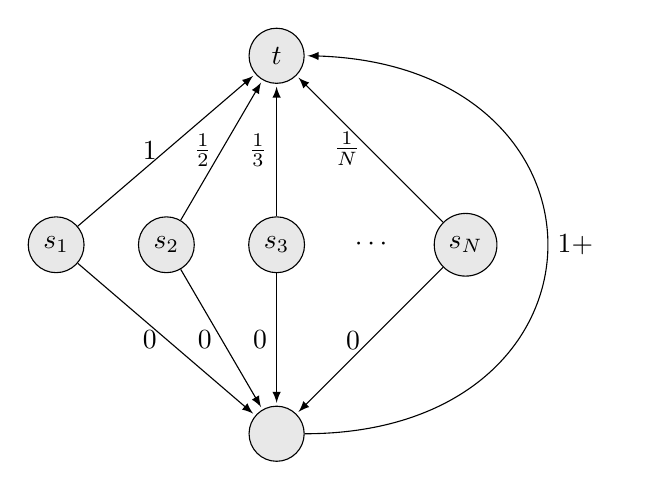
\begin{tikzpicture}[shorten >=1pt, auto,scale=0.8]
				\tikzstyle{every state}=[fill={rgb:black,1;white,10}, minimum size=0.7cm]
	\node[state] (0) at (-3.5,0)                {$s_1$};
	\node[state] (1) at (-1.75,0)                {$s_2$};
	\node[state] (2) at (0,0)                {$s_3$};
	\node (3) at (1.5,0)                {$\cdots$};
	\node[state] (4) at (3,0)                {$s_N$};
	\node[state] (5) at (0,3)                {$t$};
	\node[state] (6) at (0,-3)                {};
\path[-latex] (0) edge node[left]{$1$} (5);
\path[-latex] (1) edge node[left]{$\frac12$} (5);
\path[-latex] (2) edge node[left]{$\frac13$} (5);
\path[-latex] (4) edge node[left]{$\frac1N$} (5);
\path[-latex] (0) edge node[left]{$0$} (6);
\path[-latex] (1) edge node[left]{$0$} (6);
\path[-latex] (2) edge node[left]{$0$} (6);
\path[-latex] (4) edge node[left]{$0$} (6);
\path[-latex] (6) edge[bend right=90, looseness=2.2] node[right]{$1+\eps$} (5);

			\end{tikzpicture}
	\end{center}

		Consider the GCG with $N$ players drawn on the left where for each player $i\in[N]$,  $t_i=t$. 		The optimal cost for this GCG is when every player goes to $t$ using the edge with $0$ weight and then the edge with cost $1+\eps$. Hence the total optimal cost is $1+\eps$.
		
		Now we will calculate the best $\pne$. The only $\pne$ is when every player uses the direct  edge with cost $\frac1i$ for each  player $i\in[N]$. Therefore total cost is $H_N$. Hence $\pos$ is $\frac{H_N}{1+\eps}\geq H_N$.
\end{proof}
\begin{lemma}{}{}
	The $\pos$ of any $GCG$ with $N$ players is at most $H_N$.
\end{lemma}
\begin{proof}
	Suppose $\Gm$ be any GCG. Let $f$ be any strategy profile and $f^*$ minimizes $\Phi$. Hence $f^*$ is an $\pne$ and $\Phi(f^*)\leq \Phi(f)$. Then we have $$C(f)=\sum\limits_{\substack{e\in E\\ n_e(f)>0}}c_e=\frac1{H_N}\sum\limits_{\substack{e\in E\\ n_e(f)>0}}c_eH_N\geq \frac1{H_N}\sum\limits_{\substack{e\in E\\ n_e(f)>0}}c_eH_{n_e(f)}=\frac1{H_N}\Phi(f)\geq \frac1{H_N}\phi(f^*)$$Now  $\forall \ f'\in S$ we have $$\Phi(f')=\sum\limits_{\substack{e\in E\\ n_e(f')\geq 1}}c_eH_{n_e(f')}\geq \sum\limits_{\substack{e\in E\\ n_e(f')\geq 1}}c_e=C(f')$$Therefore we get $C(f)\geq \frac1{H_N}C(f^*)$. Hence $\pos(\Gm)\leq H_N$.
\end{proof}

\nt{The general form of argument for potential games goes like this: If $\alpha C(s)\leq \Phi(s)\leq \beta C(s)$, then $\pos\leq \frac{\beta}{\alpha}$ }

Therefore with these two lemmas we get the final theorem:
\begin{Theorem}{}{}
	The $\pos$ of any Global Connection Games with $N$ players is the  $H_N$ where $H_N$ is $N^{th}$ harmonic number.
\end{Theorem}

\chapter{Price of Anarchy Bounds in Smooth Games}
\section{Facility Location Game}
\begin{definition}{Facility Location Game}{}
	A Facility Location Game consists of \begin{enumerate}[label=(\roman*)]
		\item There is a set $L$, of $n$ locations.
		\item $SP$ is the set of $k$ service providers or players.
		\item Player $i\in SP$ has its strategy set some $S_i\subseteq L$. For player $i$, $S_i$ represents the places where player $i$ might build a facility. For some player $i\in SP$, it may also be the case that $S_i=\emptyset$, i.e. player $i$ prefers nowhere.
		\item A set $C$ of $m$ clients. 
		\item Each client $j\in C$ has some value $\pi_j\geq 0$. Think of this as how much the client is willing to pay for the service that the facilities provide.
		\item For all $l\in L$ and $j\in C$ let $c(l,j)$ is the transportation cost.
		\item For all $i\in SP$ and $j\in C$ let $p(i,j)$ is the price of $i$ for serving $j$.
	\end{enumerate}
\end{definition}


\begin{assumption}We will have the following assumptions for the game:
	\begin{itemize}
		\item $c(l,j)\neq c(l',j)$ for all $l,l'\in L$, $l\neq l'$ and $j\in C$.
		\item $\pi_j\geq c(l,j)$ for all $l\in L$ and $j\in C$.
	\end{itemize}
\end{assumption}
\subsection{Utilities: Definition}
We will define the utilities of client and service providers. Let $s\in S$ be any strategy profile. If a client $j\in C$ chooses the service provider $i\in SP$  then we denote $SP(j)=i$. 

So for any client $j\in C$ the utility for strategy profile $s$ is $$u_j(s)=\pi_j-p(SP(j),j)$$  and for  any service provider $i\in SP$, the utility of $i$ is $$u_i(s)=\sum\limits_{j\colon SP(j)=i}p(i,j)-c(s_i,j)$$ Now we define the utilitarian social welfare for a strategy profile $s$ to be $$V(s)=\sum\limits_{i\in SP}u_i(s)+\sum\limits_{j\in C}u_j(s)=\sum\limits_{j\in C}\pi_j-c\lt(s\st_{SP(j)},j\rt)$$
To make the utilities of every service provider to be non-negative we have another assumption:
\begin{assumption}
	For any strategy profile $s$, $\forall\ i\in SP$ and $\forall\ j\in C$, $p(i,j)\geq c(s_i,j)$
\end{assumption}
\begin{remark}
	This social welfare considers the clients as players as well but with simple strategies choosing the least price service provider
\end{remark}

\subsection{Choosing Prices}
Note that technically prices too are chosen by the service providers. However we will show that given a strategy profile the prices are fixed at equilibrium.

Now the service provider $i$ at location $s_i$ can get profit from client $j\in C$ only if it's the closest i.e. transportation cost satisfies $c(s_i,j)\leq c(l,j)$ for all $j\in L$.  Any client $j\in C$ chooses the service provider $i\in SP$ if the price charged by the $i$ to $j$ is minimum i.e. $p(i,j)=\min\limits_{i'\in SP}p(i',j)$.
\begin{observation*}
	For any client $j\in C$ and any service provider $i\in SP$ in a strategy profile $s$,  $SP(j)=i$ if \begin{enumerate}[label=(\roman*)]
		\item $i\in \arg\min\limits_{i'\in SP}p(i,j)$
		\item $c(s_i,j)=\min\limits_{i'\in SP}c(s_{i'},j)$
	\end{enumerate}
\end{observation*}

\begin{lemma}{}{}
	For any client $j\in C$ and any service provider $i\in SP$ in a strategy profile $s$,  $SP(j)=i$ if\begin{enumerate}[label=(\roman*)]
		\item $c(s_i,j)=\min\limits_{i'\in SP}c(s_{i'},j)$
		\item $p(i,j)=\max\lt\{c(s_i,j),\min\limits_{\substack{i'\in SP\\ i'\neq i'}}c(s_{i'},j)\rt\}$
			\end{enumerate}
\end{lemma}
\begin{proof}
	The first condition directly follows from the observation.  We will prove the second one.   Let $\hat{i}=\arg\min\limits_{i'\neq i}c(s_{i'},j)$. Suppose $c(s_i,j)<c(s_{\hat{i}},j)$. Then we have to show $p(i,j)=c(s_{\hat{i}},j)$.  
	
	Since the service providers want to maximize their utility they want to maximize the price charged to client. Now if $p(i,j)\neq c(s_{\hat{i}},j)$ then we can assume $p(i,j)>c(s_{\hat{i}},j)$. If $p(i,j)>c(s_{\hat{i}},j)$ then if $p(\hat{i},j)=\frac12\lt(p(i,j)+c(s_{\hat{i}},j)\rt)$ then $p(\hat{i},j)<p(i,j)$. Hence $SP(j)=\hat{i}$ but we are given $SP(j)=i$. Hence contradiction \ctr Hence we have the lemma.
\end{proof}
\subsection{Potential Game}
We will now show that Facility Location Game is a potential game. We will take the function $V$ which is the total utilitarian social welfare as the potential function of the game. And we will show now that this follows the condition of potential games.
\begin{Theorem}{}{}
	For any strategy profile $s$, for all $i\in SP$, $\forall\ s_i'\in S_i$ $$V(s_i',s_{-i})-V(s)=u_i(s_i',s_{-i})-u_i(s)$$
\end{Theorem}


\section{Smooth Games}

\section{Load Balancing Game}
\chapter{Introduction to Mechanism Design}

%\bibliographystyle{alpha}
%\bibliography{algorithms_refs}

\end{document}
